\documentclass[10 pt]{article}
\usepackage[a4paper, total={7in, 9.5in}]{geometry}
\usepackage[spanish]{babel}
\usepackage{csquotes}
\usepackage{graphicx} 
\usepackage{caption}
\usepackage{hyperref}
\usepackage{graphicx}
\usepackage{float}
\usepackage{url}
\usepackage{color}
\usepackage{siunitx}
\usepackage{hhline}
\usepackage{multirow}
\usepackage[round]{natbib}
\bibliographystyle{plainnat}
\usepackage{todonotes}
\linespread{1.5}
\usepackage{imakeidx}
\makeindex[columns=3, title=Alphabetical Index, intoc]
%\usepackage{amsmath}
\begin{document}




\listoftodos

\begin{titlepage}

    \begin{center}
    \vspace*{-0.5in}
    \begin{figure}[htb]
    \begin{center}
    
\includegraphics[scale=.3]{images/uba2.jpg}
    \end{center}
    \end{figure}
    
    \begin{large}
    Maestría en Explotación de Datos y Descubrimiento del Conocimiento\\
    \vspace*{0.15in}
    Universidad de Buenos Aires \\
    
    \vspace*{0.6in}
    \end{large}
    
    \begin{large}
    Trabajo integrador\\
    
    
    \end{large}
    \vspace*{0.2in}
    \vspace*{0.3in}
    
    
    \vspace*{0.3in}
    \rule{80mm}{0.1mm}\\
    \vspace*{0.1in}
    \begin{large}
    Victoria Colombo
    
    \vspace*{0.3in}
    
    \vspace*{0.1in}fecha
    \end{large}
    \end{center}
    
    \end{titlepage}

\newpage

\begin{abstract}


\end{abstract}
\newpage
\tableofcontents
\newpage

\section{Introducción}\label{intro}

\subsection{Antecedentes}


La violencia sexual comprende una multiplicidad de conductas o intentos de conductas, que van desde actos hasta comentarios sexuales, dirigidos contra la sexualidad de otra persona de manera coercitiva. El trabajo con datos sobre violencia sexual presenta complicaciones porque los datos suelen ser escasos o presentar gran cantidad de faltantes \citetext{\citealp[p.~150]{ferris2002world}}. Uno de los motivos es que las víctimas o su entorno a menudo se rehúsan a denunciar o participar en encuestas sobre este tipo de agresiones, o proveen información incompleta. Esto puede deberse a la vergüenza y el estigma social frecuentemente asociado no solo con la violencia sexual sino con la sexualidad en general, pero también a la falta de acceso a la justicia, al temor a las represalias por parte de los agresores, o el temor a que la denuncia no sea creída \citep*{murphy2022unfounded}. Otros posibles motivos para la escasez y/o mala calidad de los datos pueden ser la falta de vías adecuadas para recabar esta información, o la negligencia o desconocimiento de procedimientos adecuados por parte de oficiales de policía encargados de recibir denuncias. A pesar de las dificultades en la recolección de datos, diversos estudios a nivel mundial logran identificar patrones frecuentes en la violencia sexual. Para este trabajo, resultan relevantes dos de ellos: la mayoría de las víctimas son mujeres, mientras que los perpetradores suelen ser hombres \citetext{\citealp[p.~149]{ferris2002world}; \citealp[p.~15]{contreras2016violencia}}; y en la mayoría de los casos, los agresores son personas conocidas por las víctimas, como parejas, exparejas u otros conocidos \citetext{\citealp[p.~9]{garcia2005multi},\citealp[p.~22]{unicef2018analisis}, \citealp[p.~151]{ferris2002world}}.
 
La clasificación de las identidades de género de víctimas y perpetradores es compleja. Por un lado, muchos estudios clasifican a las personas únicamente como hombres o mujeres, omitiendo las identidades de género disidentes.\footnote{Entre los estudios e informes consultados para este trabajo, solamente el \textit{Relevamiento de fuentes secundarias de datos sobre violencia sexual} de la \citet{ufem_relevamiento} menciona identidades de género cuando especifica que la violencia sexual “afecta particularmente a las mujeres cis y personas LGBTI+” (p.7).}. Por otro lado, aunque se reportan pocos casos de violencia sexual contra hombres cisgénero, es probable que estén subrepresentados debido a los prejuicios y estigmas sociales sobre la masculinidad que dificultan las denuncias y el acceso a la justicia para estas víctimas \citep*[p.~149]{ferris2002world}. Analizar esas complejidades excede a este trabajo de especialización. En mi análisis las categorías de género de víctimas, victimarios y llamantes se limitan a las registradas en el \textit{dataset}: hombre, mujer, y transgénero, sin especificar si es un hombre o una mujer transgénero. Reconozco esto como una limitación no solo de mi trabajo sino también de los datos disponibles.  

La  recopilación, sistematización, y análisis de datos sobre violencia sexual por parte de los Estados es crucial para planificar y llevar adelante políticas efectivas de prevención, asistencia, y erradicación de la violencia sexual. En Argentina, si bien no hay un sistema estatal único y centralizado de este tipo de información, existen entidades judiciales y programas estatales que, además de ofrecer auxilio, asistencia y/o acceso a la justicia, recaban datos sobre violencia sexual, y mantienen un registro público de ellos. Unos de esos programas es Las Víctimas contra las Violencias. 

Desde el año 2016, en el marco del programa Las Víctimas contra las Violencias, dependiente del Ministerio de Justicia de la Nación, la línea 137 funciona las 24 horas del día para solicitar asistencia en casos de violencia sexual o familiar\footnote{Además, desde 2020 cuenta también con el canal de \textit{Whatsapp} (54911) 3133-1000.}. El programa cuenta con equipos de intervención de abogadas, psicólogas, y trabajadoras sociales. Al recibir una llamada solicitando asistencia se coordina el envío de equipos móviles para proveer a la víctima, en base a las necesidades del caso, de contención emocional, acompañamiento a un hospital y/o a radicar una denuncia, y/o a un lugar seguro donde pueda alojarse \citep*{linea_137}.\todo[inline]{rever cómo sigue el programa ahora}

Los registros de las llamadas a la línea 137 se encuentran digitalizados desde 2017 y están disponibles en el \href{http://datos.jus.gob.ar/}{Portal de Datos Abiertos de la Justicia Argentina}. Allí se encuentran publicados cuatro tipos de \textit{datasets}: 

\begin{itemize}
    \item Llamados por situaciones de violencia familiar
    \item Llamados por situaciones de violencia sexual
    \item Intervenciones domiciliarias por situaciones de violencia familiar
    \item Intervenciones domiciliarias por situaciones de violencia sexual
\end{itemize}

En este trabajo analizo llamados a la línea 137 para reportar violencia sexual entre 2017 y 2021. Los registros  presentan datos faltantes de dos maneras: celdas vacías en algunas variables numéricas, y respuestas no-sabe/no-contesta en lugar de sí o no en algunas variables categóricas. De particular interés para este trabajo es la variable \textit{victima\_convive\_agresor}, que codifica la situación convivencial entre la víctima y el agresor, y toma los valores \textit{SI}, \textit{NO}, y \textit{NS/NC}.

\subsection{Objetivos}

Mis objetivos para este trabajo son:

\begin{itemize}
    \item Analizar los datos para determinar si existen patrones y asociaciones que permitan caracterizar a la población de víctimas que convive con su agresor y la que no lo hace.
    \item Entrenar un modelo predictivo que trate como datos faltantes las respuestas \textit{NS/NC} en la variable \textit{victima\_convive\_agresor} y los clasifique como \textit{SI} o \textit{NO}. 
    \item En particular, entrenar un modelo de Máquinas de Soporte Vectorial.\footnote{En adelante, \textit{SVM} por sus siglas en inglés: \textit{Support Vector Machine}.}  
    \item Contrastar dos tipos de preprocesamientos de los datos para entrenar el modelo: el primero utilizando el método de ordenamiento y reducción de dimensionalidad de Escalamiento Multidimensional No-Métrico.\footnote{En adelante, \textit{NMDS} por sus siglas en inglés \textit{Non-Metric Multidimensional Scaling}; el segundo, reduciendo dimensiones de los datos de manera manual,a través de la eliminación, agrupación y transformación de las variables.}

\end{itemize}


\section{Datos}\label{datos}

\subsection{Obtención y limpieza}\label{limpieza}
Descargué del \href{http://datos.jus.gob.ar/}{Portal de Datos Abiertos} mencionado arriba 5 \textit{datasets} en formato \textit{csv} de llamados a la línea 137 para solicitar asistencia por violencia sexual. Los archivos pertenecen, a razón de uno de por año, al período entre enero de 2017 y julio de 2021. 

Una vez descargados, unifiqué los 5 archivos en un solo \textit{dataset}. Para eso fue necesario realizar una primera limpieza destinada a dejar consistentes los distintos archivos en términos de cantidad y nombre de columnas\footnote{La limpieza, normalización, y preprocesamiento del \textit{dataset} y la aplicación de los métodos exploratorios y predictivos fueron realizados en Python}:

\begin{itemize}
    \item Eliminé la variable \textit{caso\_id}, que solo existe a partir de 2020.
    \item Cambié el nombre de la variable \textit{llamado\_provincia\_indec\_id} en los \textit{datasets} de 2017, 2018, y 2019 a su equivalente en 2020 y 2021: \textit{llamado\_provincia\_id}.
\end{itemize}

El siguiente paso fue limpiar el \textit{dataset} unificado de inconsistencias y errores de carga varios: 
\begin{itemize}
    \item Unifiqué para todas las variables pertinentes los valores \textit{SI}, \textit{NO}, y \textit{NS/NC} dejándolos en mayúscula, ya que aparecían en distintos formatos: minúscula, mayúscula inicial, etc.
    \item Unifiqué en la variable \textit{victima\_vinculo\_agresor} el valor \textit{Ex pareja de la víctima} que aparecía también como \textit{Ex pareja}, \textit{Ex-pareja de la víctima} y \textit{Expareja de la víctima}, otro tanto hice con \textit{Pareja de la víctima} que presentaba variaciones similares.
    \item Unifiqué en \textit{hecho\_lugar} dos variaciones de una misma categoría: \textit{Otra institución}, y \textit{Otra Institución}, optando por la primera forma.
    \item Sustituí todos los valores \textit{Sin datos} por \textit{NS/NC} por considerarlos equivalentes.
    \item Quité espacios de comienzo y final de \textit{strings} para solucionar problemas del tipo \textit{Madre} =/= \textit{  Madre} 
    \item Convertí en la variable \textit{llamante\_vinculo} el valor \textit{Vecino} a \textit{Vecina/o}, ya que  no necesariamente se refiere unívocamente a personas de género masculino.
    \item Unifiqué en \textit{llamado\_provincia} “Ciudad Autónoma de Buenos Aires” y “CABA” optando por “CABA”. 
    \item Corregí en \textit{llamado\_provincia }las instancias de “Santa Fé” a “Santa Fe”.

\end{itemize}

\subsection{Exploración}\label{exploración}

El \textit{dataset} final unificado consta de 19143 observaciones y 54 variables, en su mayoría categóricas, que aportan información sobre la víctima, el agresor, la persona que llama para reportar el hecho, el contexto del hecho y el tipo de violencia sufrida. En el cuadro \ref{tablavar} se puede ver un detalle de las variables y su tipo.

\begin{table}[H]
    \centering
    \caption{Resumen de las variables.}
    \label{tablavar}
    \begin{tabular}{|l|l|l|} 
    \hline
    \textbf{Descriptor} & \textbf{Tipo variable} & \textbf{Variable(s)}         
    \\ 
    \hline
    \multirow{2}{*}{Víctima} & Cuantitativa & victima\_edad 
    \\ 
    \cline{2-3}
     & Cualitativa & \begin{tabular}[c]{@{}l@{}}victima\_genero, victima\_nacionalidad, victima\_discapacidad, \\ victima\_vinculo\_agresor, victima\_convive\_agresor, victima\_a\_resguardo\end{tabular}          
     \\ 
    \hline
    \multirow{2}{*}{Llamante} & Cuantitativa         & {llamante\_edad}             
    \\ 
    \cline{2-3}
     & Cualitativa& llamante\_genero, llamante\_vinculo                  
     \\ 
    \hline
    \multirow{2}{*}{Llamado}& Ordinal & llamado\_fecha\_hora                                            
    \\ 
    \cline{2-3} & Cualitativa & \begin{tabular}[c]{@{}l@{}} caso\_id, llamado\_provincia llamado\_provincia\_id, \\ caso\_judicializado, hecho\_lugar\end{tabular}                                
    \\ 
    \hline
    Violencia sexual                 & Cualitativa  &  \begin{tabular}[c]{@{}l@{}} vs\_violacion\_via\_vaginal, vs\_violacion\_via\_anal, vs\_violacion\_via\_oral, \\ vs\_tentativa\_violacion, vs\_tocamiento\_sexual, vs\_intento\_tocamiento, \\ vs\_intento\_violacion\_tercera\_persona, vs\_grooming, vs\_exhibicionismo, \\ vs\_amenazas\_verbales\_contenido\_sexual, vs\_explotacion\_sexual,\\ vs\_explotacion\_sexual\_comercial, vs\_explotacion\_sexual\_viajes\_turismo, \\ vs\_sospecha\_trata\_personas\_fines\_sexuales, \\ vs\_existencia\_facilitador\_corrupcion\_nnya, \\ vs\_obligacion\_sacarse\_fotos\_pornograficas, vs\_eyaculacion\_partes\_cuerpo, \\ vs\_acoso\_sexual, vs\_iniciacion\_sexual\_forzada\_inducida, \\ vs\_otra\_forma\_violencia\_sexual, vs\_no\_sabe\_no\_contesta \end{tabular} 
    \\ 
    \hline
    Otras violencias & Cualitativa & \begin{tabular}[c]{@{}l@{}} ofv\_sentimiento\_amenaza, ofv\_amenazas\_explicitas, ofv\_violencia\_fisica, \\ ofv\_intento\_ahorcar, ofv\_intento\_quemar,  ofv\_intento\_ahogar, \\ ofv\_amenaza\_muerte, ofv\_uso\_sustancias\_psicoactivas, \\ ofv\_intento\_privacion\_libertad, ofv\_privacion\_libertad, \\ ofv\_uso\_arma\_blanca, ofv\_uso\_arma\_fuego, ofv\_enganio\_seduccion,\\ ofv\_intento\_matar, ofv\_uso\_animal\_victimizar, ofv\_grooming, \\ ofv\_otra\_forma\_violencia, ofv\_no\_sabe\_no\_contesta\end{tabular} 
    \\ 
    \hline
    \end{tabular}
\end{table}

Las variables que describen la violencia sexual sufrida y otras formas de violencia reportadas pueden tomar los valores \textit{SI} o \textit{NO}, siendo este último el valor más común, como se aprecia más abajo en las figuras \ref{vssino} y \ref{ofvsino} que muestran la distribución de respuestas para violencia sexual y otras formas de violencia respectivamente. Es interesante notar el volumen de respuestas positivas de las categorías \textit{vs\_no\_sabe\_no\_contesta} y \textit{ofv\_no\_sabe\_no\_contesta}. Es decir, en gran cantidad de llamados se reporta una forma de violencia (sexual o no) sufrida, pero no se puede reportar qué forma. A lo largo de esta sección se observa esta prevalencia de respuestas de tipo \textit{NS/NC} en casi todas las variables.

\begin{figure}[H]
\begin{center}
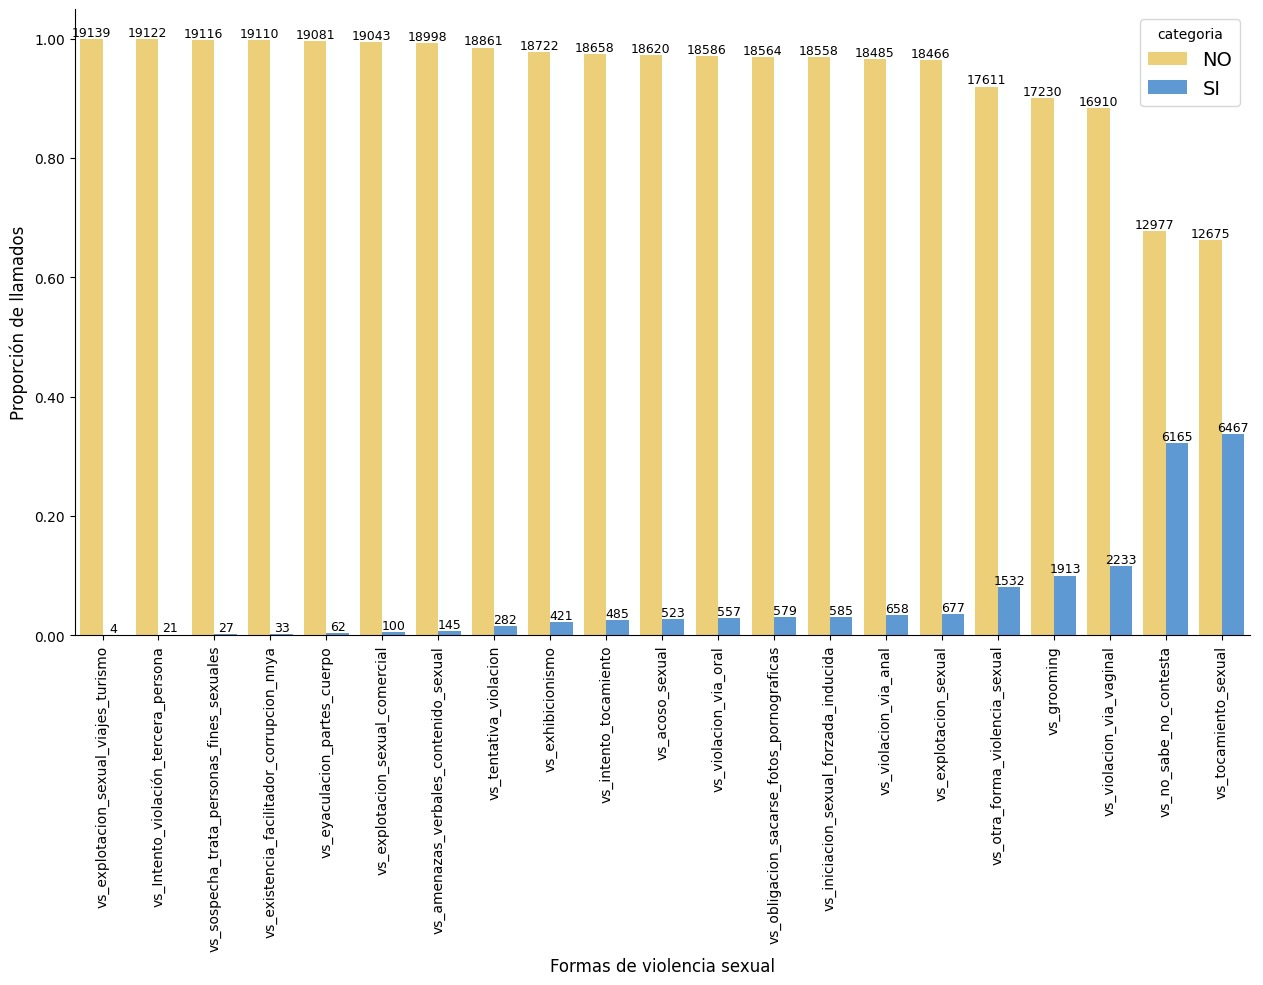
\includegraphics[scale=.5]{images/latex_vs_sino.jpeg}
\caption{Tipos de violencia sexual reportada en los llamados.}
\label{vssino}
\end{center}
\end{figure} 

\begin{figure}[H]
\begin{center}
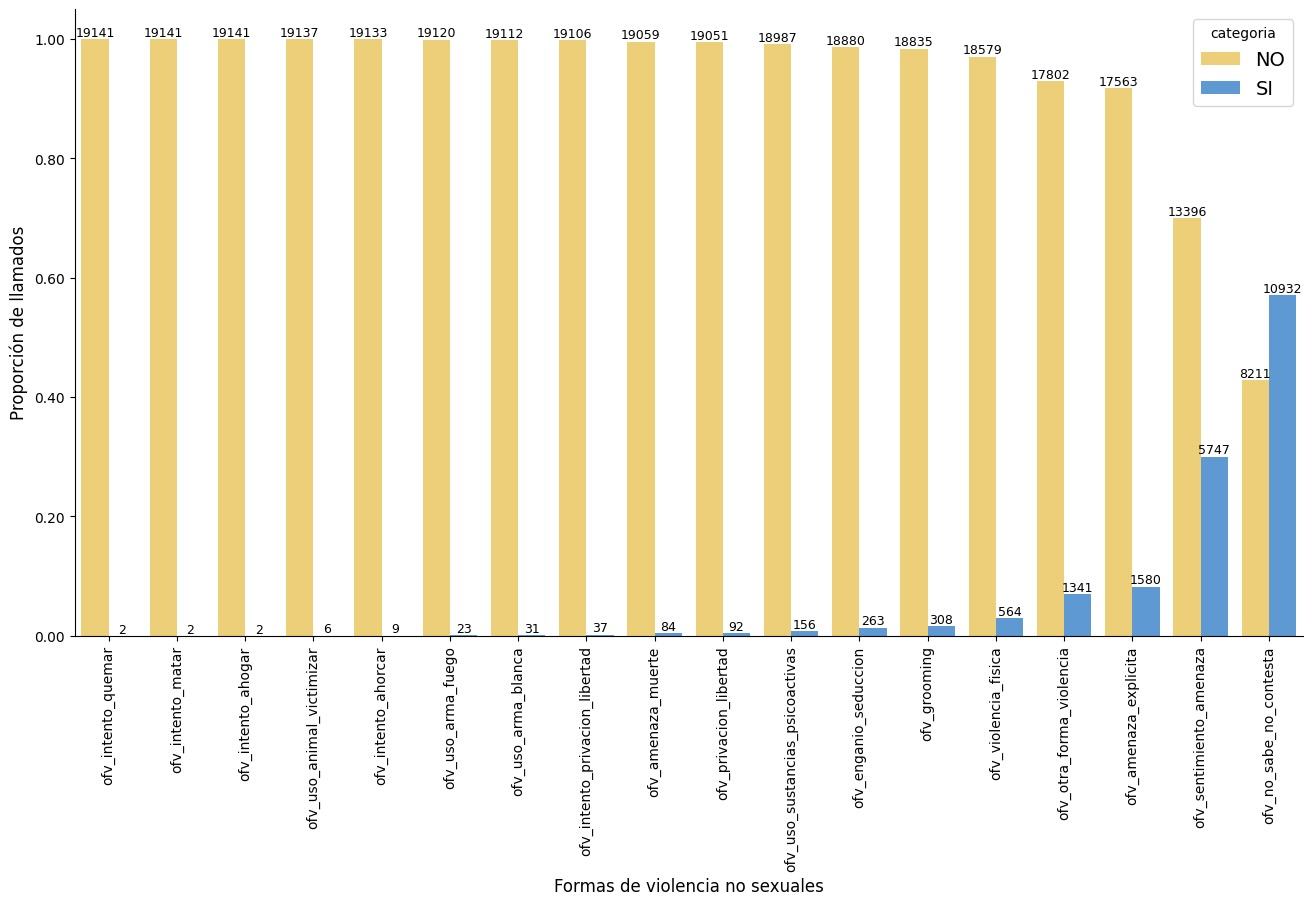
\includegraphics[scale=.5]{images/latex_ofv_sino.jpeg}
\caption{Tipos de violencia no sexual reportada en los llamados.}
\label{ofvsino}
\end{center}
\end{figure} 



Las variables \textit{victima\_edad} y \textit{llamante\_edad} presentaban valores atípicos positivos, no solo identificables por superar la barrera de \(3*IQR\), sino también y principalmente por ser valores incongruentes con la edad de una persona. Por lo tanto, removí todos los valores por encima de 110 para ambas variables, y todos los valores por debajo de 1 para \textit{llamante\_edad} (si existen víctimas que presentan edad 0, considero que se trata de menores que aún no alcanzan el año). Los valores removidos y su cantidad para cada variable pueden verse en el cuadro 2, \nameref{tabla_out}. Se puede comprobar allí que la mayoría eran 999 en ambas variables, muy probablemente un valor por defecto ingresado para no dejar el campo vacío. En total, removí 195 valores en \textit{llamante\_edad}, y 101 valores en \textit{victima\_edad}. 


\begin{table}[H] 
    \centering
    \caption{Outliers en variables de edad.}
    \label{tabla_out}
    \begin{tabular}{|l|c|c|}
    \hline
    \textbf{Variable}                        & \textbf{Outlier} & \textbf{Cantidad de filas} \\ \hline
    \multirow{2}{*}{llamante\_edad} & 999     & 192               \\ \cline{2-3} 
                                    & 0       & 3                 \\ \hline
    \multirow{4}{*}{victima\_edad}  & 999     & 98                \\ \cline{2-3} 
                                    & 224     & 1                 \\ \cline{2-3} 
                                    & 125     & 1                 \\ \cline{2-3} 
                                    & 111     & 1                 \\ \hline
    \end{tabular}
    \end{table}

Una vez removidos estos valores, tomé las medidas descriptivas de las variables de edad que se observan en el cuadro \ref{tabla_descr_ed}. Se puede ver que la mayoría de las víctimas no supera los 21 años, con una media de 17 y una moda de 14. Las personas que llaman para reportar los casos, en cambio, son en su mayoría adultos, con una media de 36 años, y una moda de 40. Esto refuerza lo mencionado en la introducción de hallazgos de otros estudios de que las personas más jóvenes y sobre todo los adolescentes e infantes son los grupos más en riesgo de ser víctimas de violencia sexual. 



    \begin{table}[H]
        \centering
    \caption{Medidas descriptivas de las variables de edad.}
    \label{tabla_descr_ed}
        \begin{tabular}{lcc}    
        \hline
        \textbf{Descriptor} & \textbf{Edad de quien llama} & \textbf{Edad de la víctima} \\ \hline
        Media               & 36.25                        & 17.17                       \\
        Moda                & 40                           & 14                          \\
        Desvío Est.     & 11.41                        & 11.91                       \\
        Min.                & 3                            & 0                           \\
        25\%                & 29                           & 10                          \\
        50\%                & 35                           & 14                          \\
        75\%                & 42                           & 21                          \\
        Max                 & 99                           & 99                          \\ \hline
        \end{tabular}
        \end{table}


Para explorar patrones en la distribución temporal de los llamados realicé el gráfico de tendencia de la figura \ref{trend} con los datos agregados mensualmente y una media móvil de 4 meses. Se puede ver claramente en este gráfico una tendencia creciente en la cantidad de llamados desde mediados de 2017, que podría estar asociada a campañas de concientización sobre el programa y la línea y también sobre la violencia doméstica en general. Hay picos de llamados que se repiten alrededor de finales de cada año, entre los meses de octubre y enero en 2016, 2017, 2018 y 2020 aunque no parecen ser consistentes en tamaño como para considerarlos una tendencia clara. Por otro lado, hay una gran suba entre finales de 2018 y comienzos de 2019 que puede estar asociada a factores externos como los que mencioné antes. Se observa, luego de una baja y período de estabilización en 2019, una suba marcada en 2020. Un factor externo que podría estar relacionado con este patrón, es la implementación de políticas de ASPO (Aislamiento Social Preventivo y Obligatorio) durante la epidemia de COVID-19 de 2020 que obligó a la población a permanecer en sus hogares y entornos más cercanos. Si tenemos en cuenta la mayor prevalencia de la violencia sexual en ámbitos cercanos y por parte de agresores conocidos a la víctima, podría explicarse la suba de cantidad de llamados durante esta época. Sin embargo, cabe aclarar, que todas las posibles asociaciones que planteo como interpretación de esta figura deben ser contrastadas con un análisis en profundidad de las series temporales del \textit{dataset}, que excede los objetivos de este trabajo.

\begin{figure}[H]
    \begin{center}
    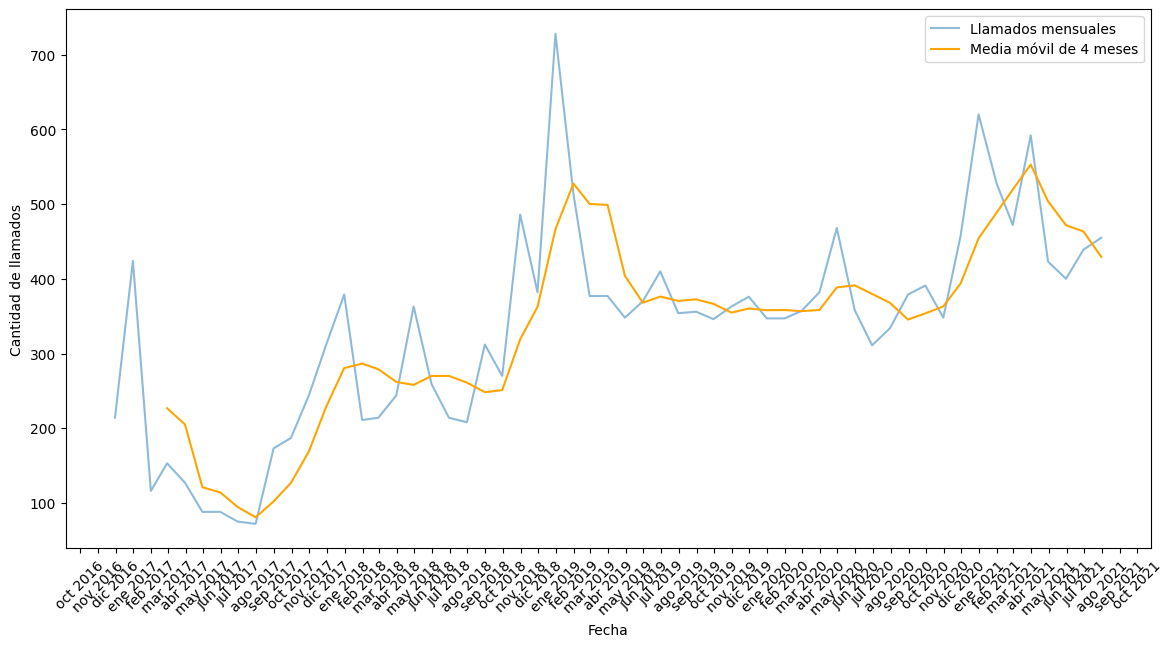
\includegraphics[scale=.5]{images/latex_trend_llamados.png}
    \caption{Cantidad de llamados en el tiempo con media móvil de 4 meses.}
    \label{trend}
    \end{center}
    \end{figure}

Además, construí las variables \textit{estación del año}, \textit{fin de semana}, y \textit{momento del día} para explorar la posibilidad de otros patrones en los llamados. Observé que una mayor proporción de llamados ocurren durante la semana (80\%) y por la tarde (38\%). No observé disparidad significativa en la distribución de llamados de acuerdo a las estaciones del año.


Según la distribución de la variable \textit{llamado\_provincia}, la mayoría de los llamados provienen de la Ciudad Autónoma (37\%) y la Provincia de Buenos Aires (36\%). Del 9\% no se cuentan con datos (respuestas \textit{NS/NC}); y el restante 18\% se reparte entre las restantes provincias del país, siendo de ese grupo Córdoba y Santa Fé las que más llamados tienen, con un 3\% cada una.\footnote{Ver figura \ref{provincia} en el \nameref{anex}.}

Según la distribución de la variable \textit{caso\_judicializado}, el 46.7\% de los llamados no está asociado a un caso ya judicializado, el 39.7\% sí, y en el restante 13.4\% no se cuenta con datos de este tipo.\footnote{Ver figura \ref{casojudicializado} en el \nameref{anex}.} 

En cuanto a la variable \textit{hecho\_lugar}, como ilustra el gráfico de barras de la figura \Ref{hecholugar}, para aproximadamente el 30\% de los llamados no se cuenta con datos (respuestas \textit{NS/NC}); luego, el 25\% los hechos suceden en la vivienda de la víctima y el 13\% en la vivienda del agresor. La cuarta categoría más reportada, con el 12\%, es \textit{redes sociales}. El restante 20\% se divide entre categorías de espacios públicos (plazas, descampados, etc.), transporte, y ámbito educativo, entre otros sitios. La elevada proporción de casos que suceden en la vivienda de la víctima, es un dato que acompaña lo ya dicho en la \nameref{intro} sobre la mayoría de los hechos de violencia sexual ocurriendo más bien en el entorno de la víctima antes que involucrar personas y lugares desconocidos. 

\begin{figure}[H]
    \begin{center}
    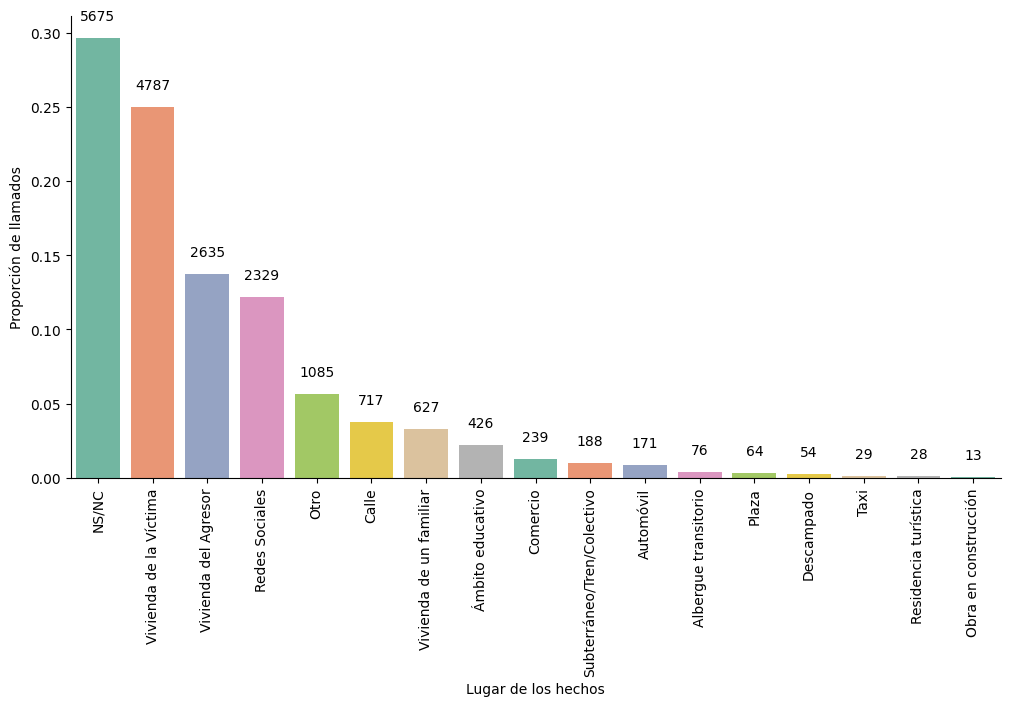
\includegraphics[scale=.5]{images/latex_lugar_hechos.png}
    \caption{Lugar de los hechos.}
    \label{hecholugar}
    \end{center}
    \end{figure}


Llama la atención la cuarta categoría más presente en \textit{hecho\_lugar}, los casos sucedidos en redes sociales. Dada la media de edad de las víctimas que reporté más arriba, se podría hipotetizar sobre la relación entre estas variables: la población joven pasa más tiempo en redes sociales y entonces es más propensa a sufrir violencia sexual en ese lugar; o las redes sociales son lugares donde proliferan más los actos de violencia sexual por alguna(s) característica(s) intrínseca(s) de las redes mismas. 

%Para explorar este fenómeno, crucé en la figura \ref{redes}  esa categoría de \textit{hecho\_lugar} con los tipos de violencia sufrida y las edades de las víctimas agrupadas cualitativamente en Niñez (0 a 11 años), Adolescencia (12 a 18 años), Juventud (19 a 30 años), Adultez (31 a 65 años), y Vejez (mayores de 65). Observé que la mayor cantidad de casos corresponden al tipo de violencia \textit{grooming} en primer lugar, y en segundo lugar a la categoría \textit{ofv\_no\_sabe\_no\_contesta}. Además, aunque con conteos mucho más bajos, aparecen también otras formas de violencia esperables en el contexto de redes sociales como: \textit{ofv\_sentimiento\_amenaza}, \textit{vs\_explotacion\_sexual}, o \textit{ofv\_amenaza\_explicita}. En todos estos casos alrededor del 90\% de las víctimas son niñes o adolescentes. Si bien por la distribución de la variable \textit{victima\_edad} cabría esperar mayor cantidad de víctimas de estos grupos etarios, en el caso de los hechos sucedidos en redes sociales, este dato podría estar asociado con el mayor uso de redes sociales por parte de este sector de la población. 

%\begin{figure}[H]
%    \begin{center}
%    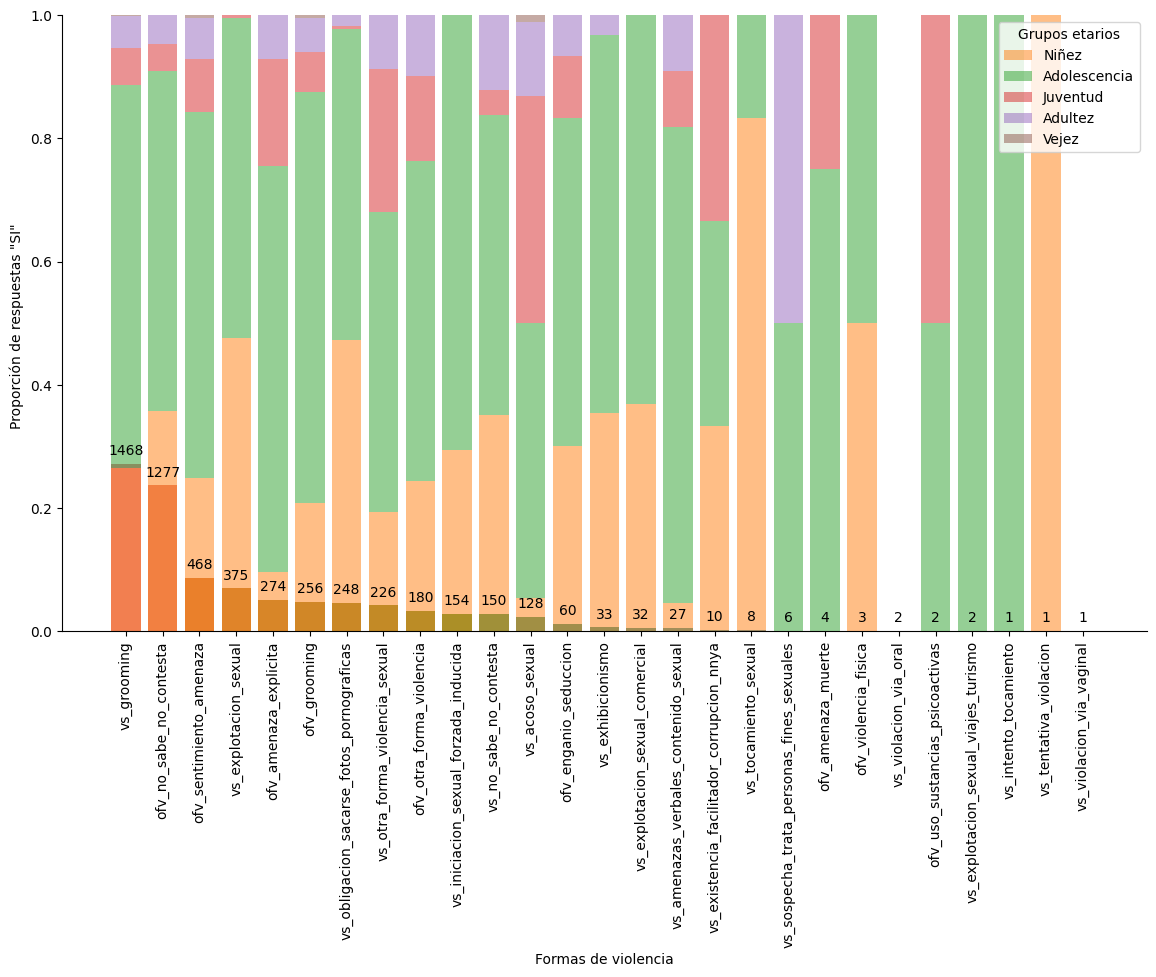
\includegraphics[scale=.5]{images/latex_redes_sociales_edad_formas_violencia.png}
%    \caption{Proporción de “SI” en hechos de violencia ocurridos en redes sociales, agrupado por edad.}
%    \label{redes}
%    \end{center}
%    \end{figure}


La nacionalidad de las víctimas, informada por \textit{victima\_nacionalidad}, se distribuye de la siguiente manera: el 80\% de las víctimas son argentinas; del 15\% no se cuenta con datos; y el restante 5\% se divide entre las nacionalidades boliviana, paraguaya, peruana, brasileña, uruguaya, chilena, y la categoría “otra”.\footnote{Ver figura \ref{nacionalidad} en el \nameref{anex}}
\todo[inline]{reduje víctima nacionalidad para SVM?}

Según la distribución de \textit{victima\_discapidad}, para el 53.7\% de las víctimas no se cuenta con datos, el 43.2\% no posee discapacidad, y el 2.9\% sí\footnote{Ver figura \ref{discapacidad} en el \nameref{anex}}. 


En cuanto al género de las víctimas, en el gráfico de barras de la figura \Ref{genero}, se ve reforzado lo establecido en la Introducción sobre la distribución de género en las víctimas: el 77.6\% de las víctimas son mujeres, el 18.4\% hombres, del 3.7\% no se tienen datos, y el 0.14\% son personas transgénero. 

\begin{figure}[H]
    \begin{center}
    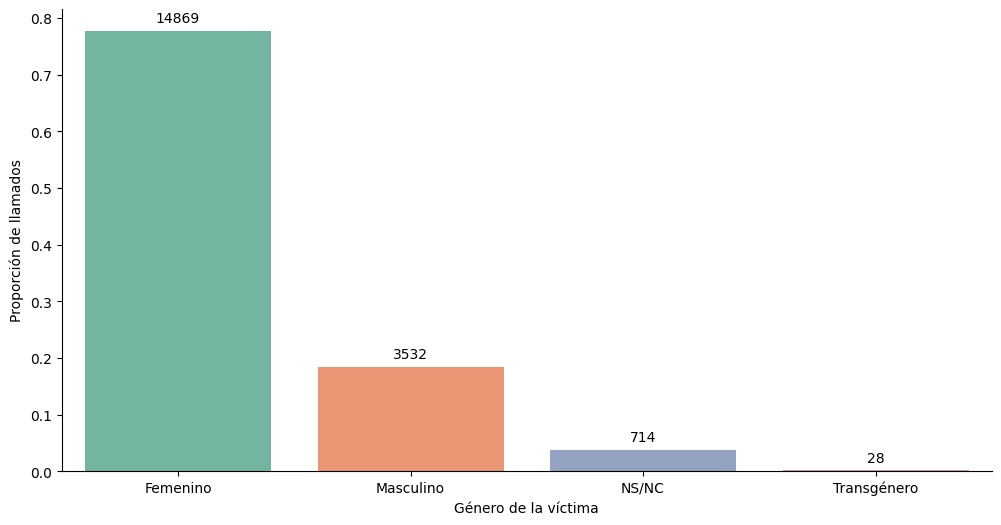
\includegraphics[scale=.5]{images/latex_genero_victima.png}
    \caption{Género de las víctimas.}
    \label{genero}
    \end{center}
    \end{figure}

Los vínculos entre víctimas y agresores nuevamente reflejan la persistencia de los hechos de violencia sexual perpetuados por personas del entorno de las víctimas. En el gráfico de barras de la figura \Ref{vinculoagresor} para la variable \textit{victima\_vinculo\_agresor} se observa la distribución en las diferentes categorías vinculares. Pero además la tendencia se evidencia aún más al reagrupar las categorías de la variable en \textit{Conocido familiar}, \textit{Conocido no familiar} (categoría ya presente en la variable original) \textit{Desconocido}, y \textit{NS/NC}. Mientras que 15.4\% de los agresores son declarados como desconocidos; entre familiares (47.4\%) y no familiares (19.7\%), los agresores conocidos por la víctima suman un 67.1\%. El número podría incluso ser más elevado si consideramos que podría haber agresores conocidos también como parte del 17.2\% de los \textit{NS/NC}.



\begin{figure}[H]
    \begin{center}
    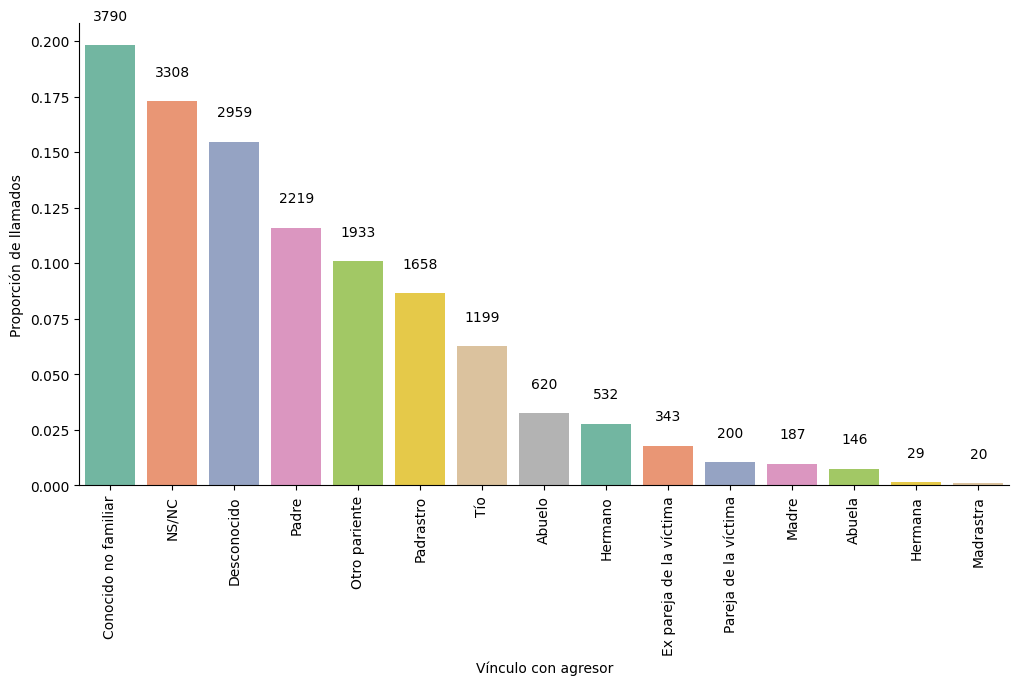
\includegraphics[scale=.5]{images/latex_vinculo_agr_victima.png}
    \caption{Vínculos víctima-agresor.}
    \label{vinculoagresor}
    \end{center}
    \end{figure}

    \begin{figure}[H]
        \begin{center}
        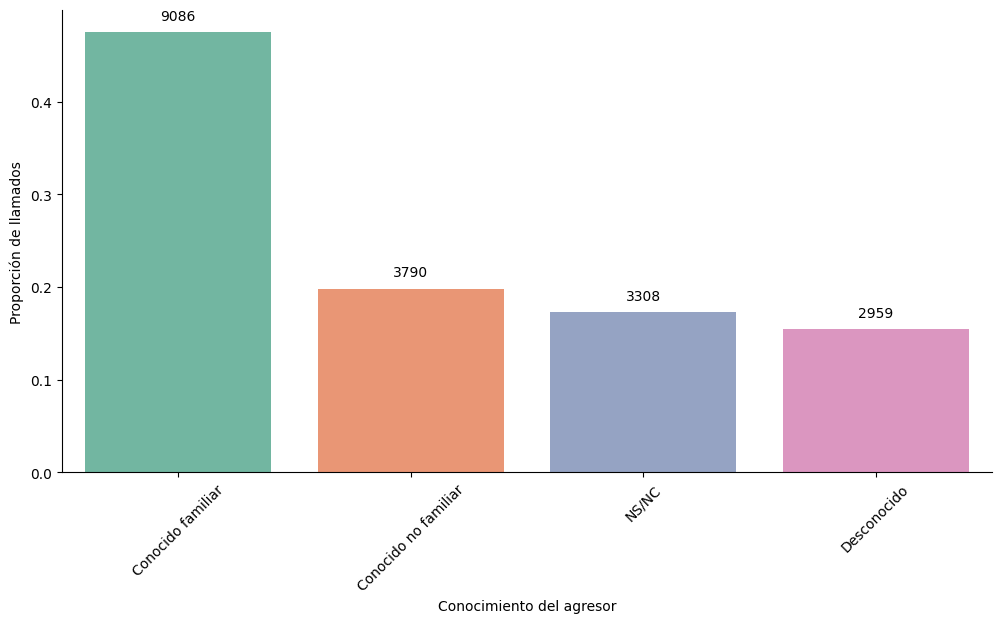
\includegraphics[scale=.5]{images/latex_agresor_conocido_no.png}
        \caption{Agresor conocido o no por la víctima.}
        \label{conocidodesconocido}
        \end{center}
        \end{figure}




 En la variable \textit{vinculo\_llamante\_victima}, el 24.9\% de los llamados provienen de comisarías, el 17.2\% de un familiar de la víctima (otro familiar que no pertenezca a las categorías: \textit{Madre}, \textit{Padre}, \textit{Abuela/o}, o \textit{Hermana/o}), el 16\% de los llamantes son madres de las víctimas, y el 14.2\% lo constituyen las propias víctimas. El resto de las categorías son otros conocidos de las víctimas, padres, vecinos, abuelos, hermanos, otras instituciones, o \textit{NS/NC} todas con menos del 10\%. Por último, los llamados provenientes de escuelas, defensorías y los mismos agresores suman menos del 1\%.\footnote{Ver figura \ref{vinculollamante} en el \nameref{anex}}



En cuanto a la variable de interés \textit{victima\_convive\_agresor}, encontré en el análisis univariado que puede verse en el gráfico de barras de la figura \Ref{convivencia}, que quiénes sí conviven con su agresor son minoría, 14.3\%; mientras que el 64.4\% no convive con su agresor. El restante 21.19\% las respuestas son \textit{NS/NC}, la categoría que más adelante intento predecir como \textit{SI} o \textit{NO}.  


\begin{figure}[H]
    \begin{center}
    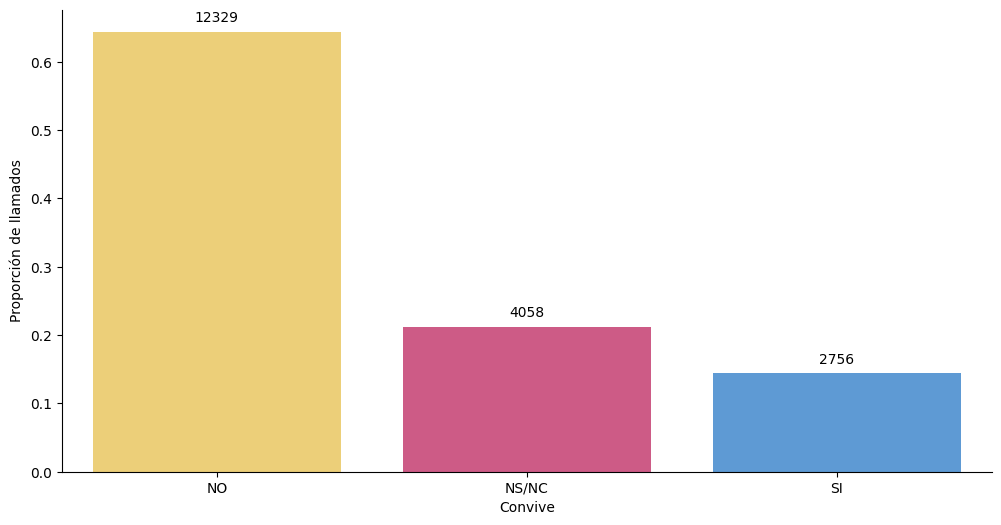
\includegraphics[scale=.5]{images/latex_convive.png}
    \caption{Convivencia víctima-agresor.}
    \label{convivencia}
    \end{center}
    \end{figure}


\subsubsection{Análisis multivariado de \textit{victima\_convive\_agresor}}\label{faltantes}


Para un análisis multivariado seleccioné algunas variables que podían estar más relacionadas con \textit{victima\_convive\_agresor}: 
\textit{hecho\_lugar}, \textit{momento\_dia}, \textit{victima\_vinculo\_agresor}, \textit{llamante\_vinculo}, y \textit{victima\_edad}. 

Primero, realicé gráficos de barras para explorar la relación entre \textit{victima\_convive\_agresor} y las variables categóricas.
Observé que la distribución original de \textit{victima\_convive\_agresor} (mayoría de respuestas \textit{NO} y minoría de \textit{SI}, con \textit{NS/NC} posicionado ordinalmente en el medio), se mantiene para casi todas las categorías de estas variables con las siguientes excepciones. En primer lugar, como se ve en la figura \ref{hecholugconvive}, cuando los hechos suceden en la vivienda de la víctima, hay más casos en los que la víctima sí convive con el agresor y la distribución pasa a ser \textit{NO}, \textit{SI}, \textit{NS/NC}. Lo mismo sucede cuando los hechos ocurren en la vivienda del agresor, aunque en ese caso la proporción de \textit{SI} supera por muy poco la proporción de \textit{NS/NC}. 

En segundo lugar, en la figura \ref{agrvincconvive} se observa que para la mayor parte de los casos en los que el agresor es parte de la familia de la víctima (\textit{Abuelo}, \textit{Hermana}, \textit{Hermano}, \textit{Madrastra}, \textit{Madre}, \textit{Padrastro}, \textit{Pareja de la víctima}), los casos en que la víctima convive son más que los casos en los que no hay respuesta sobre la situación convivencial. Sin embargo, solo en las categorías \textit{Madre}, \textit{Padrastro}, y \textit{Pareja de la víctima} los casos en que las víctimas conviven con sus agresores superan a los casos en los que no lo hacen.

Por último, en la figura \ref{llamvincconvive}, se puede ver que para la categoría \textit{vecina/o} de \textit{llamante\_vinculo}, la tendencia de respuestas positivas y negativas también se invierte. Sobre esta variable se observa además que los valores de \textit{NS/NC} para \textit{victima\_convive\_agresor} son notablemente más altos cuando el llamado proviene de \textit{Otra institución} que no sea una escuela, comisaría, u hospital. 


\begin{figure}[H]
\begin{center}
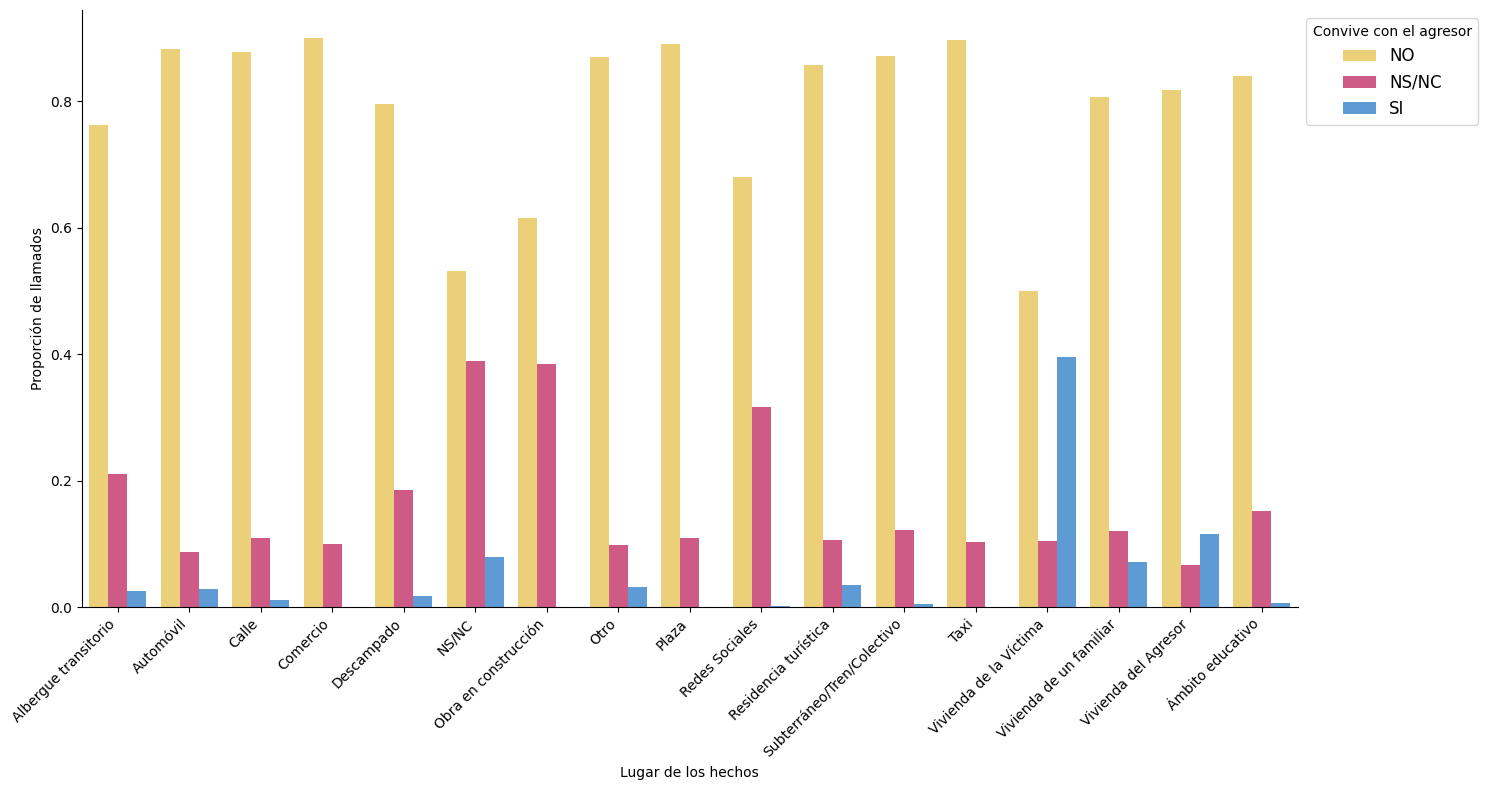
\includegraphics[scale=.5]{images/latex_hecho_lugar_convive.png}
\caption{Convivencia con el agresor según lugar de los hechos.}
\label{hecholugconvive}
\end{center}
\end{figure}
    
\begin{figure}[H]
\begin{center}
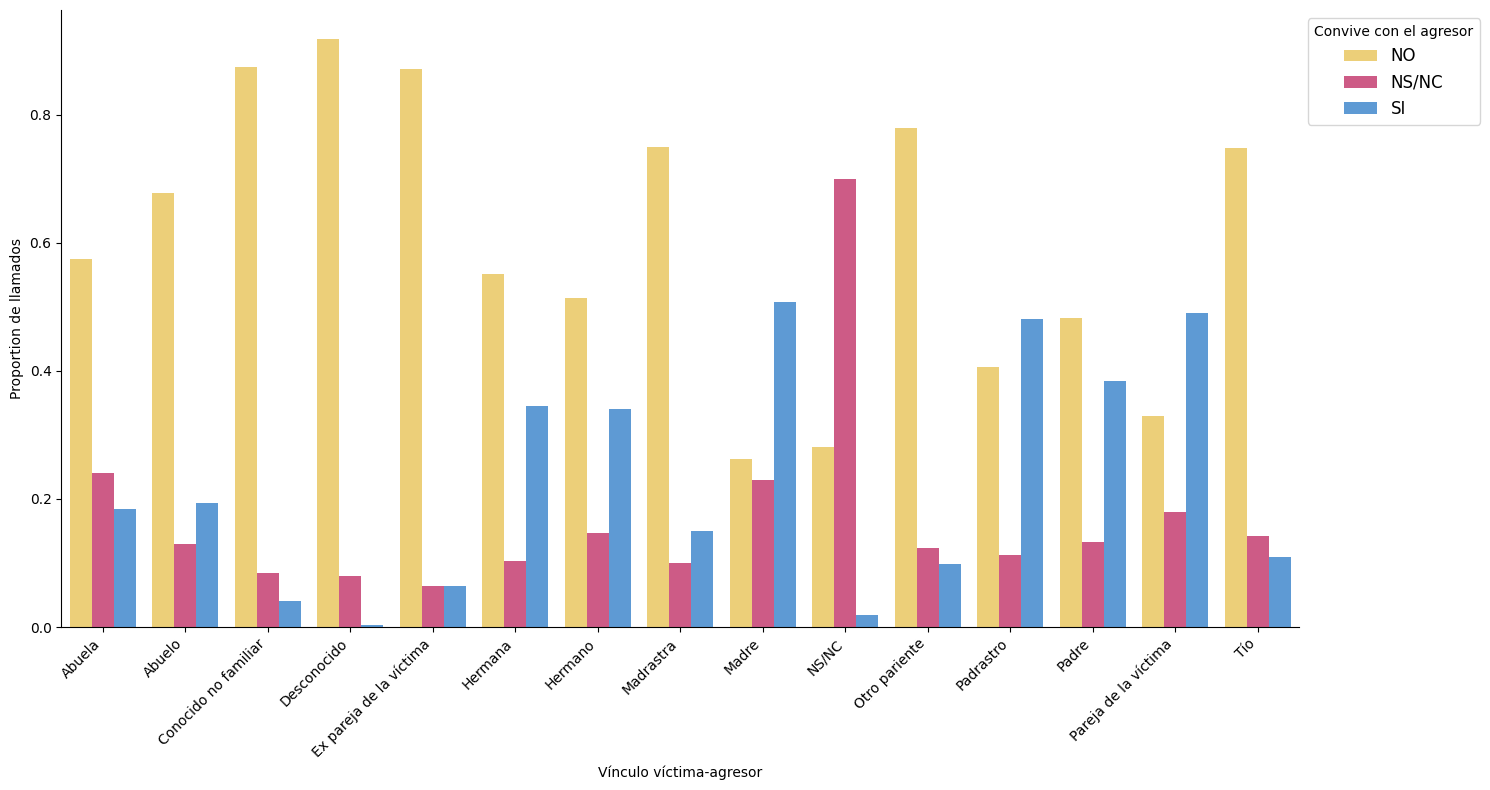
\includegraphics[scale=.5]{images/convive_vinc_agresor.png}
\caption{Convivencia con el agresor según vínculos víctima-agresor.}
\label{agrvincconvive}
\end{center}
\end{figure} 

\begin{figure}[H]
\begin{center}
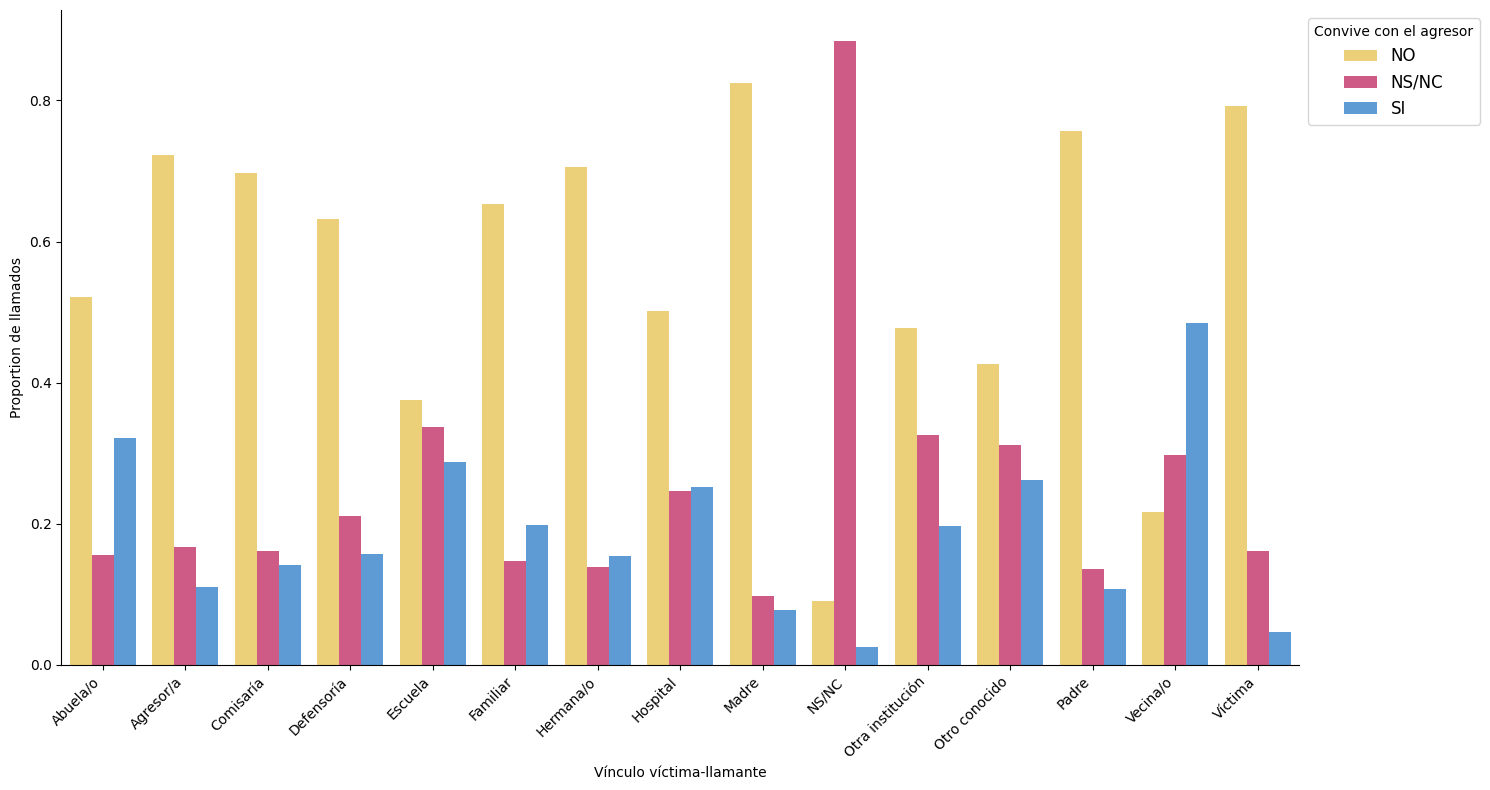
\includegraphics[scale=.5]{images/latex_llamante_vin_convive.png}
\caption{Convivencia con el agresor según vínculos víctima-llamante.}
\label{llamvincconvive}
\end{center}
\end{figure} 


Luego realicé \textit{boxplots} comparativos y un detalle del análisis de cuartiles de \textit{victima\_edad} según cada categoría de \textit{victima\_convive\_agresor}. Como se ve en la figura \ref{boxplotsconvivenciaedad} y el cuadro \ref{cuartilesconviveedad}, las víctimas que conviven con el agresor son ligeramente más jóvenes que las que no lo hacen; y las víctimas de las que no se cuenta con datos sobre la convivencia parecen estar más cerca en edad de las que conviven. Sin embargo, estas diferencias en edad no parecen significativas\footnote{Realizo en la sección \nameref{met} un análsis más detallado con respecto a la correlación estadística entre la edad de la víctima y la variable de convivencia, entre otras.}. 

\begin{figure}[H]
    \begin{center}
    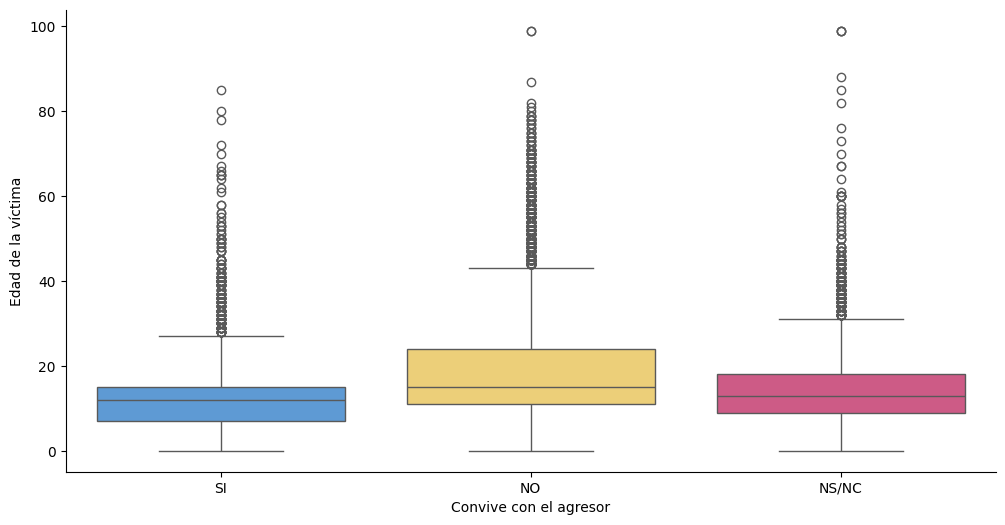
\includegraphics[scale=.5]{images/latex_boxplot_convive_edad.png}
    \caption{Distribución de la edad de la víctima según su convivencia o no con el agresor.}
    \label{boxplotsconvivenciaedad}
    \end{center}
    \end{figure}


\begin{table}[H]
    \begin{center}
    \caption{Cuartiles de edad según categoría de \textit{victima\_convive\_agresor}.}
    \label{cuartilesconviveedad}
    \begin{tabular}{cccc}
    \hline
    \multicolumn{1}{r}{\textbf{}} & \textbf{Convive} & \textbf{No Convive} & \textbf{ NS/NC} \\ \hline
    Q1                            & 7                    & 11                   & 9                       \\
    Media                         & 12                   & 15                   & 13                      \\
    Q3                            & 15                   & 24                   & 18                      \\
    IQR                           & 8                   & 13                   & 9                     \\ \hline
    \end{tabular}
    \end{center}
    \end{table}


Evalué también una posible relación entre la edad de la víctima, el vínculo con el agresor, y la situación de convivencia o no con este. En la figura \ref{edadconvagr} se observa la tendencia que ya se presentó en los \textit{boxplots} de \ref{boxplotsconvivenciaedad}: las medias de edades de las víctimas según sus situaciones convivenciales con el agresor son similares entre sí. Destaco, sin embargo, que para las categorías \textit{Pareja} y \textit{Ex-pareja de la víctima} la media de edad de las víctimas es ligeramente más alta en comparación a las otras categorías de vínculos; y que específicamente la media de edad de las víctimas que sí conviven con sus agresores es más alta que la de las que no conviven o aquellas para las que no se cuenta con datos sobre la convivencia. La media de edad también se dispara para la categoría vincular \textit{Madrastra} en los casos en que no se tienen datos sobre la situación convivencial. Por último, quiero señalar que las medias de edad más bajas ocurren con agresores \textit{Abuelo}, \textit{Abuela}, \textit{Madrastra}, y \textit{Padre}, donde ninguna media de edad supera los 10 años en las víctimas que sí conviven con sus agresores.

\begin{figure}[H]
    \begin{center}
    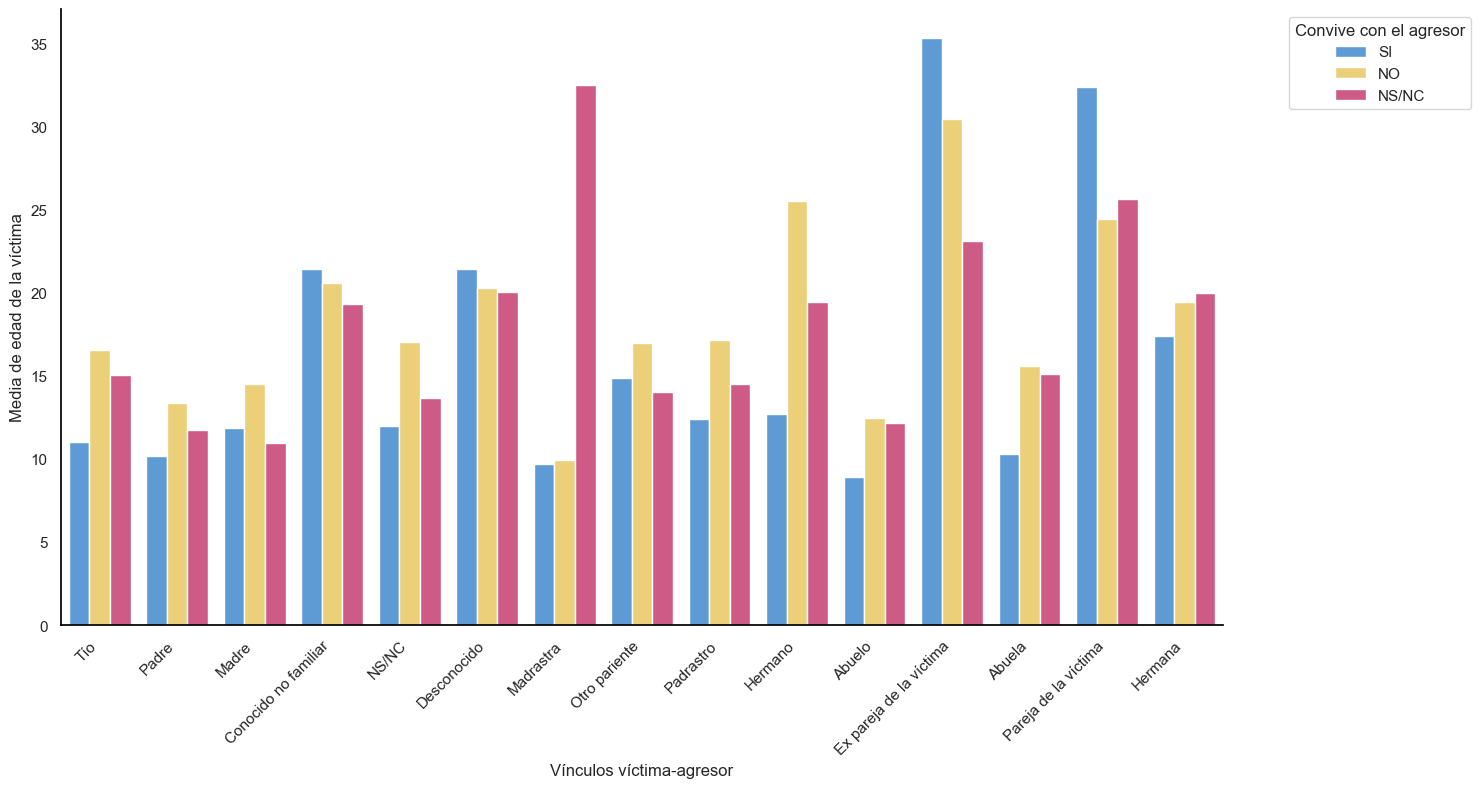
\includegraphics[scale=.4]{images/convive_edad_agresor.png}
    \caption{Edad de la víctima según su vínculo y convivencia o no con el agresor.}
    \label{edadconvagr}
    \end{center}
    \end{figure}


Por último, puse en relación \textit{victima\_convive\_agresor} con los valores faltantes en \textit{victima\_edad}, que representan el 9.82\%. Apliqué al conjunto de datos un filtro para incluir solamente las filas con casos vacíos de \textit{victima\_edad}, y generé el mismo gráfico de barras de la figura \Ref{convivencia} con esos datos. El resultado, que puede verse abajo en la figura \Ref{conviveedadfaltantevic}, muestra un aumento de los casos de respuesta \textit{NS/NC} para \textit{victima\_convive\_agresor}. En \textit{dataset} completo, \textit{NS/NC} representaba el 21.19\% en \textit{victima\_convive\_agresor}, cuando solo se observan los casos con datos faltantes de edad de la víctima, ese porcentaje sube a 57.49\%. Es decir, cuando no se tienen datos sobre la edad de la víctima, tampoco se los tiene en mayor medida sobre la situación convivencial entre la víctima y el agresor.

\begin{figure}[H]
    \begin{center}
    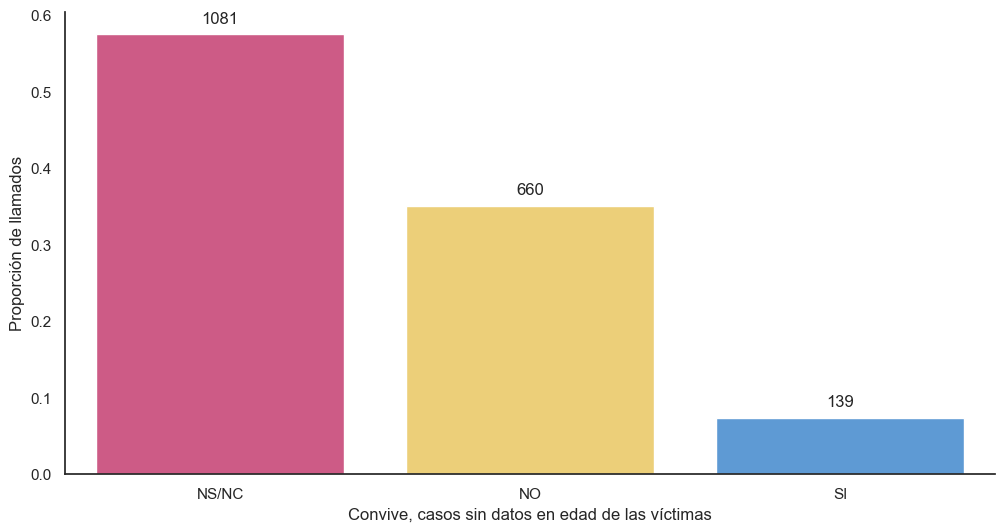
\includegraphics[scale=.5]{images/latex_convive_sd_edad_vic.png}
    \caption{Convivencia víctima-agresor en las filas de datos faltantes para \textit{victima\_edad}.}
    \label{conviveedadfaltantevic}
    \end{center}
    \end{figure}




Teniendo en cuenta la clasificación de datos faltantes que se origina en \citet{rubin1976inference}, los datos faltantes en el \textit{dataset} de llamados son posiblemente del tipo \textit{missing at random} (MAR) y \textit{missing not at random/ non-ignorable missing data} (MNAR). Es decir, o bien los datos faltan por motivos que tienen que ver con otras variables (MAR), o bien el valor faltante está relacionado con el motivo mismo por el que falta (MNAR).\todo[inline]{acá o en resultados}    


\section{Metodología}\label{met}

La gran cantidad de variables que presenta el conjunto de datos acarrea limitaciones a la hora de buscar relaciones de más de dos o tres variables con la variable de interés, y puede causar problemas de procesamiento en el entrenamiento del modelo predictivo con SVM. Para reducir las dimensiones del \textit{dataset} aplico un preprocesamiento con NMDS, y un preprocesamiento manual de eliminación y agrupamiento de variables. La aplicación de NMDS me permite además generar visualizaciones en dos dimensiones del total del conjunto. La reducción manual de las variables presenta sus propios desafíos e implicó también una reducción de la cardinalidad de algunas para mitigar problemas de \textit{encoding}. Finalmente entreno modelos predictivos de SVM con \textit{datasets} generados con los dos tipos de preprocesamientos y con otras variaciones necesarias para solventar los datos numéricos faltantes en las variables de edad.


\subsection{Reducción de los datos con NMDS}

 El NMDS se utiliza a menudo como método de ordenamiento para mostrar similitudes y diferencias entre los datos a través de representarlos en espacios de bajas dimensiones, priorizando que las distancias en el nuevo espacio sean fidedignas a las distancias en el espacio original de altas dimensiones \citetext{\citealp{kruskal1964nonmetric}}. 
 La aplicación de este método me permite mitigar el posible problema de procesamiento (al reducir las dimensiones de los datos), a la vez que generar visualizaciones en dos dimensiones distinguiendo los niveles de \textit{victima\_convive\_agresor} para buscar agrupamientos entre ellos que delimiten a cada clase.

Al ser un método flexible con respecto a la matriz de distancias que utiliza, me permitió calcular para mis datos la distancia de Gower, una medida de similitud que puede calcularse entre datos de distinto tipo



 Para el caso particular de NMDS

%“Let S be the similarity matrix, and X the coordinates of the n input points. Disparities dij are transformation of the similarities chosen in %some optimal ways. The objective, called the stress, is then defined by 

%\[\sqrt{\frac{\sum_{i<j} \left( d_{ij} - \hat{d}_{ij} \right)^2}{\sum_{i<j} d_{ij}^2}}\]
    








%\todo[inline]{poner fórmula Gower}. 

%A trivial solution to this problem is to set all the points on the origin. In order to avoid that, the disparities 
 %are normalized. Note that since we only care about relative ordering, our objective should be invariant to simple translation and scaling, however the stress used in metric MDS is sensitive to scaling. To address this, non-metric MDS may use a normalized stress, known as Stress-1 defined as

 De la función para MDS de sklearn me resultaron relevantes los parámetros\footnote{se utiliza una para escalamiento métrico (MDS) y se ajustan los parámetros necesarios para convertirla en escalamiento no-métrico. } 
 
 \begin{itemize}
    \item \textit{n\_dimensions}: dimensiones para variar la cantidad de dimensiones en las que al algoritmo proyecta el nuevo ordenamiento de los datos
    \item \textit{metric}: \textit{False} para el escalamiento no-métrico 
    \item \textit{dissimilarity}: para especificar la medida de similitud o diferencia a utilizar con los datos. En este caso toma el valor \item \textit{precomputed} que me permite pasarle directamente al método \textit{fit\_transform} la matriz de distancias de Gower.
    \item \textit{normalized\_stress} tRUE para la versión no métrica
 \end{itemize}

La desventaja de esta metodología es que la matriz de Gower no puede calcularse con datos vacíos, por lo tanto las variables de edad, las únicas con celdas vacías, resultaron un problema. La solución fue crear dos tipos de \textit{datasets}: uno en que la edad está categorizada y los datos faltantes clasificados como \textit{NS/NC}; y uno en que descarto la variable \textit{llamante\_edad} y trabajo únicamente con los casos completos de la variable \textit{victima\_edad}. Esta decisión que general el segundo conjunto de datos está guiada por el supuesto de que la edad de quien llama es menos relevante para la variable \textit{target} que la edad de la víctima; y por otro lado, por el hecho de que la edad de la víctima falta en el 9.82\% de los casos, mientras que la edad de quien llama falta en el 44.82\% y dejar afuera estos casos reduciría demasiado el conjunto de datos. 

Apliqué entonces NMDS sobre dos versiones del conjunto total de datos: A: edad categorizada, B: eliminación de llamante edad y solo datos completos de victima edad. Varié el parámetro n\_dimensions en disitntas iteraciones para evaluar el stress 

Tanto el entrenamiento de modelos como los gráficos de ordenamiento de los datos utilizaron las distintas versiones del dataset reducido que mencioné: datos completos con la variable edad categorizada, y una versión con la variable llamante edad eliminada y solo los casos completos de edad de la víctima. 

\subsection{Reducción manual de los datos}

 %problemas para aplicar métodos de \textit{encoding} como el \textit{one hot encoding}. %\citetext{\citealp[p.~3]{udilua2023encoding}}% 


Como se puede apreciar en los gráficos de las figuras \Ref{vssino} y \Ref{ofvsino} de la sección \nameref{datos}, muchas de las variables tienen en su mayoría respuestas \textit{NO}, por lo que resultan poco informativas. Además, muchas comparten dominio semántico y jurídico, como por ejemplo \textit{ofv\_uso\_arma\_blanca}, y \textit{ofv\_uso\_arma\_fuego}.

Reduje entonces la cantidad de variables que describen los tipos de violencias sufridas, en primer lugar, agrupando algunas de ellas en cuatro nuevas variables por dominio. En el cuadro \Ref{tablaagrup} a continuación resumo cada grupo de variables y la nueva variable que las reemplaza. 


\begin{table}[H]
    \centering
    \caption{Agrupación de variables de violencia por dominio.}
    \label{tablaagrup}
    \begin{tabular}{|c|l|}
    \hline
    \multicolumn{1}{|l|}{\textbf{Nueva variable agrupadora}} & \multicolumn{1}{c|}{\textbf{Variables agrupadas}} \\ \hline
    \multirow{4}{*}{vs\_explotación\_sexual}                 & vs\_explotación\_sexual                           \\ \cline{2-2} 
                                                             & vs\_explotación\_sexual\_comercial                \\ \cline{2-2} 
                                                             & vs\_explotación\_sexual\_viajes\_turismo          \\ \cline{2-2} 
                                                             & vs\_sospecha\_trata\_personas\_fines\_sexuales    \\ \hline
    \multirow{3}{*}{vs\_violacion}                          & vs\_violancion\_via\_vaginal                      \\ \cline{2-2} 
                                                             & vs\_violancion\_via\_anal                         \\ \cline{2-2} 
                                                             & vs\_violancion\_via\_oral                         \\ \hline
    \multirow{4}{*}{ofv\_intento\_violencia\_fatal}          & ofv\_intento\_ahogar                              \\ \cline{2-2} 
                                                             & ofv\_intento\_quemar                              \\ \cline{2-2} 
                                                             & ofv\_intento\_matar                               \\ \cline{2-2} 
                                                             & ofv\_intento\_ahorcar                             \\ \hline
    \multirow{2}{*}{ofv\_uso\_arma}                          & ofv\_uso\_arma\_blanca                            \\ \cline{2-2} 
                                                             & ofv\_uso\_arma\_fuego                             \\ \hline
    \end{tabular}
    \end{table}


En segundo lugar, eliminé las variables cuya tasa de respuesta \textit{SI} representaba menos del 1\% de los casos. 

Las variables eliminadas fueron:

\begin{itemize}
    \item \textit{vs\_amenazas\_verbales\_contenido\_sexual} 
    \item \textit{vs\_existencia\_facilitador\_corrupcion\_nnya}
    \item \textit{vs\_eyaculacion\_partes\_cuerpo}
    \item \textit{ofv\_amenaza\_muerte}
    \item \textit{ofv\_uso\_sustancias\_psicoactivas} 
    \item \textit{ofv\_intento\_privacion\_libertad}
    \item \textit{ofv\_privacion\_libertad}
    \item \textit{ofv\_uso\_animal\_victimizar} 
\end{itemize}


rEDUCCI´ON DE LA CARDINALIDAD DE LAS VARIABLES 

\subsection{Modelos SVM}

Vamos a reducirlo antes de aplicar un método predictivo. Dos maneras de reducirlo, NMDS y manual
A través del análisis que llevé a cabo durante la epxloración de los datos Con el objetivo de visualizar el dataset en dimensiones reducidas me da una
idea de agrupamientos con repsecto a las tres categorías de convive. Elijo NMDS porque me permite trabajar con
variables de distinto tipo sin transformaciones.
 Luego, para intentar predecir los NSNC como si o no usé SVM. 

A modo de un segundo preprocesamiento para poder llevar a cabo estas tareas, decidí reducir las dimensiones del dataset a mano primero agrupando variables y reduciendo la cantidad de categorías en algunas otras variables. lA REDUCCI´OND E CARDINALIDAD DE algunas variables es especialemnte útil para la aplicación de SVM ya que esta conlleva encodear las features y para uno de los encoders elegidos, one-hot, la alta cardinalidad de features puede resultar problemática.


Habiendp hecho los gráficos de más arriba para explorar posibles interacciones entre dos o tres variables, me pareció valioso explorar más dimensiones y plasmarlo en dos dimensiones. Para eso apliqué NMDS

Reducción manual de dimensiones


Despues medí correlación para ver si podía sacar más variables pero al final no saqué ninguna. Explicar cómo queda el dataset final

Después apliqué encoders para hacer SVM e hice SVM con la librería tal y con una búsqueda de hiperparámetros. Además experimenté con diferentes versiones del dataset cambiando la variable edad numérica por su contraparte categórica. Esto me peritió medir el posible impacto de los datos faltantes de edad. Cuando la edad era numérica, debía dejar afuera los datos faltantes ya que SVM no puede utilizarlos. Para poder utilizar todos los datos completos de edad, pasé la edad a categorica  utilizando las categorías tal tal y tal y dejado como NSNC los datos faltantes. Teniendo en cuenta estas variaciones en el tratamiento de la variable edad, los experimentos que realicé con SVM fueron: 
tal tal tal

cada uno probando los siguientes hiperparámentros

VER DE ARMAR UNA TABLA QUE RESUMA ESTAS VARIANTES 


\section{Resultados}\label{resultados}
NMDS vemos que no hay en ninguna de las veriones del dtaset que usé una separación clara entre las categorías de interés.

VER DE RE ARMAR NMDS y que separe solo SI de NO y luego un tercero que haga SI NO NSNC

Todos dieron bien y luego el mejor modelo lo apliqué a 

\section{Discusión y conclusiones}\label{conc}
cruzamiento de datos ovd líneas de asistencia, observatorio de género.
acceso y análisis de datos extensivo a provincias, no solo benos aitres


%VER DE EN SVM RESULTANTE FINAL A LOS QUE LES PUSO S´I CU´AL ES LA EDAD DE V´ICTIMA Y A LOS QUE LES PUSO NO, CU´AL ES

en \textit{La guerra contra las mujeres}, \citeyearpar{segato2016guerra}, Rita Segato habla de la violencia sexual como algo siempre dirigido hacia cuerpos femeninos y \textit{feminizados} (resaltado propio). Con esto último quiere decir cuerpos percibidos o construidos por los abusadores como femeninos con respecto a posiciones de poder: menores, débiles, racializados, pertenecientes a disidencias sexuales. Esto se condice con datos sobre la mayor incidencia de la violencia sexual contra identidades masculinas durante la niñez y la adolescencia, es decir, en períodos en que los cuerpos y los sujetos son más vulnerables, y por lo tanto, también percibidos como feminizados \citep*{contreras2016violencia,ufem_relevamiento,ferris2002world}.

Si las denuncias de violencia sexual contra disidencias de género representan una minoría en los datos, ¿quiere decir esto que esas personas sufren menos violencia sexual?, ¿O quiere decir que, como minoría social, están subrepresentados en general y que tienen menos acceso a la justicia?



Análisis de series temporales, porsibilidad de hacer forcasting

Las víctimas que sí conviven suelen ser más jóvenes pero por muy pocos, no a significativa la correlación, salvo en el caso de agresores parejas o ex parejas de las víctimas. Pero además hay vínculos con agresores más comuens que otros para esas víctimas que sí conviven y son jóvenes.
\newpage


\bibliography{bibtex_reporte.bib}

\newpage
\section{Anexo}\label{anex}




\begin{figure}[H]
\begin{center}
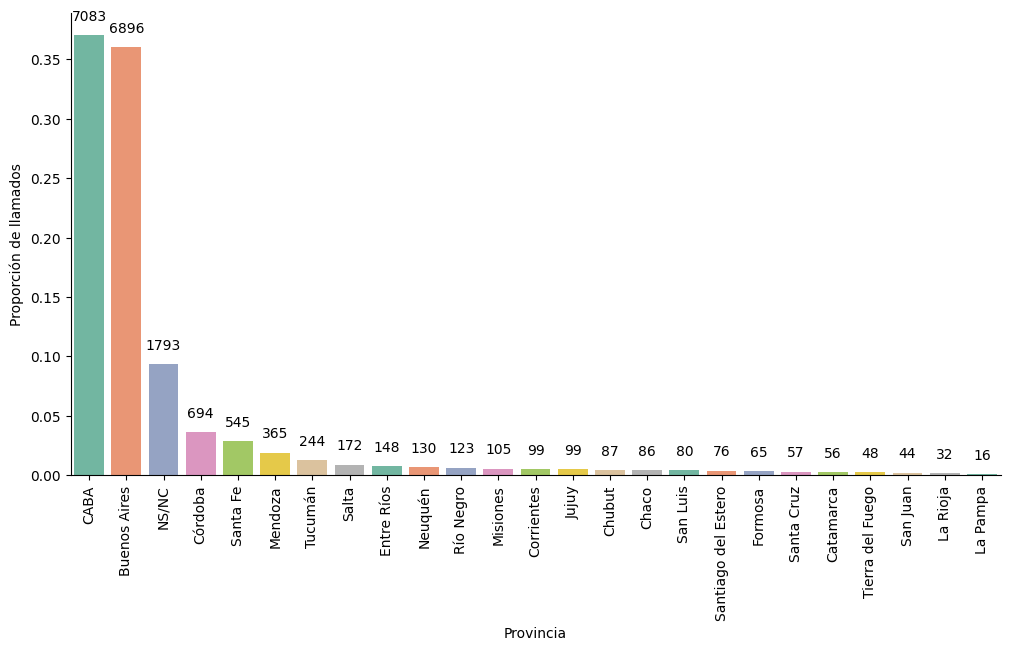
\includegraphics[scale=.5]{images/latex_llamados_por_provincia.png}
\caption{Llamados por provincia.}
\label{provincia}
\end{center}
\end{figure}

\begin{figure}[H]
\begin{center}
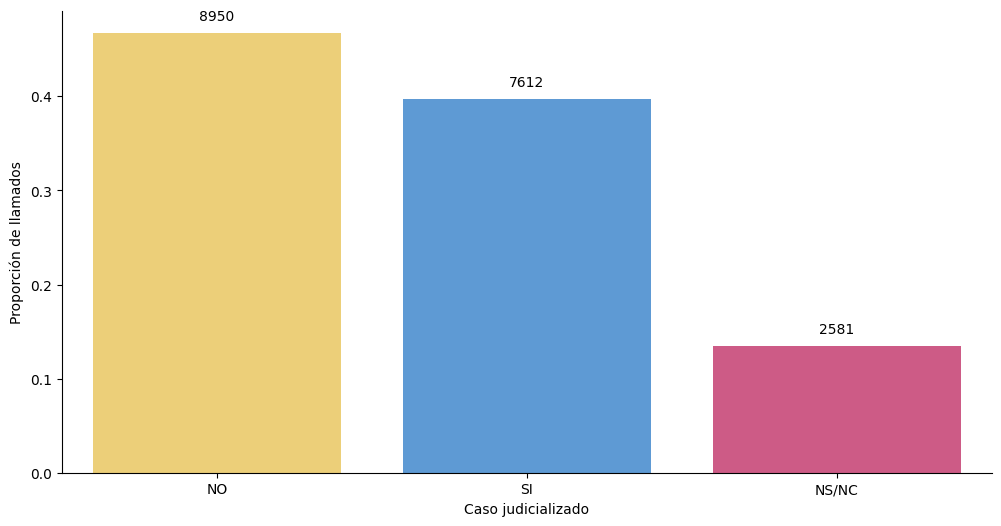
\includegraphics[scale=.5]{images/latex_caso_judicializado.png}
\caption{Caso judicializado.}
\label{casojudicializado}
\end{center}
\end{figure}


\begin{figure}[H]
\begin{center}
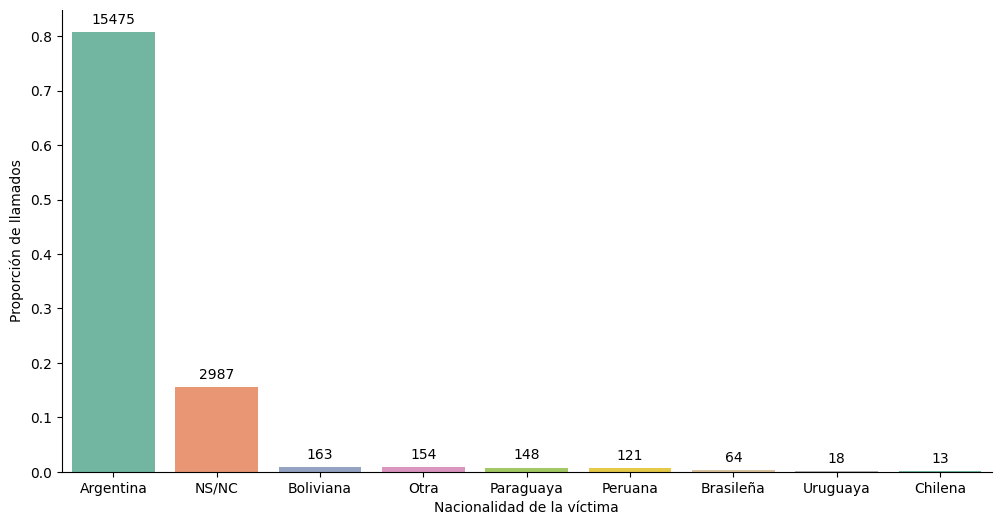
\includegraphics[scale=.5]{images/latex_nacionalidad_victima.png}
\caption{Nacionalidad de las víctimas.}
\label{nacionalidad}
\end{center}
\end{figure}



\begin{figure}[H]
\begin{center}
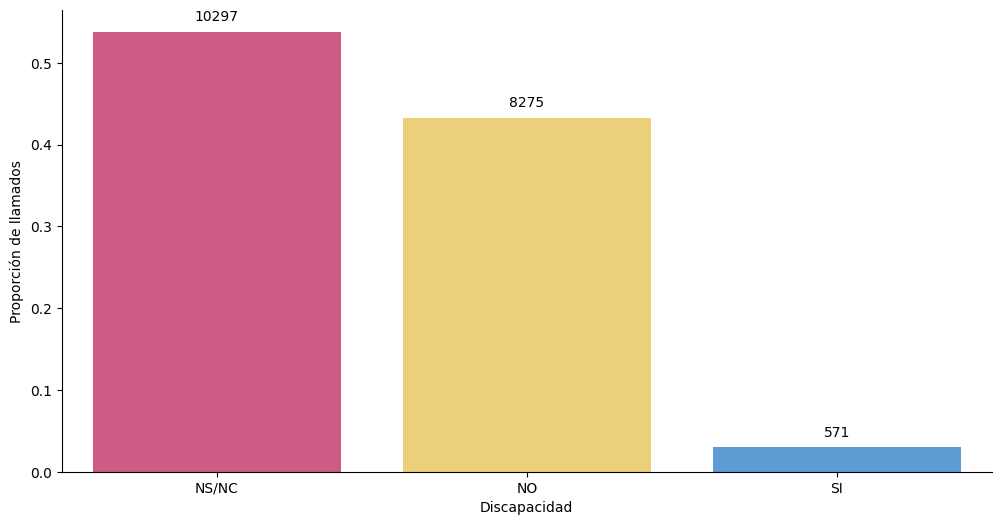
\includegraphics[scale=.5]{images/latex_victima_discapacidad.png}
\caption{Presencia de discapacidad en las víctimas.}
\label{discapacidad}
\end{center}
\end{figure}



\begin{figure}[H]
\begin{center}
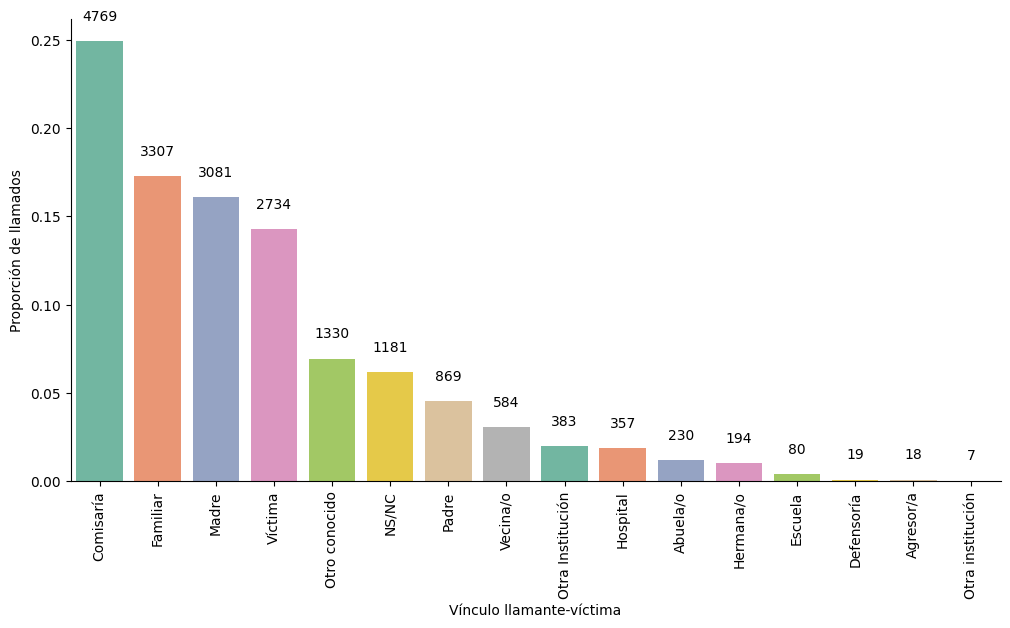
\includegraphics[scale=.5]{images/latex_vinculo_llamante.png}
\caption{Vínculos víctima-llamante.}
\label{vinculollamante}
\end{center}
\end{figure}



\end{document}